\section{Model Wienera}
Model Wienera to struktura nieliniowego systemu, w której liniowy blok dynamiczny jest umieszczony przed nieliniowym blokiem statycznym. Oznacza to, że najpierw wejście przechodzi przez liniowy filtr, a następnie poddawane jest nieliniowej transformacji. Modele Wienera są szczególnie użyteczne w systemach, gdzie obserwowana nieliniowość wynika głównie z ograniczeń lub nasycenia elementów wykonawczych, takich jak silniki, zawory, czy inne elementy mechaniczne.  Zatem istota tego modeli jest taka sama jak w przypadku modelu Hammersteina - oddzielenie nieliniowej statyki od liniowej dynamiki - z tym, że nieliniową statykę poprzedzono liniową dynamika - odwrotnie niż jak to było w przypadku omówionego modelu, co graficznie zilustrowano na rys. \ref{wien_model}.

\begin{figure}[h!]
\centering
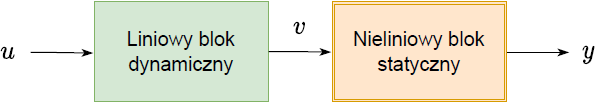
\includegraphics[width=\textwidth]{pictures/wien_model}
\caption{Reprezentacja graficzna modelu Wienera.}
\label{wien_model}
\end{figure}

Sygnał wejściowy trafia na liniowy blok dynamiczny, którego wyjściem jest przekonwertowany sygnał $v = f(u)$, który następnie trafia na nieliniową statykę, której wyjściem jest sygnał $y$.

Warto podkreślić, że modele Wienera jest trudniejszy w interpretacji niż model Hammersteina. Wynika to z tego, że sygnał wejściowy przechodzi najpierw przez system liniowy, a dopiero potem przez nieliniowy element, co utrudnia analizę wpływu nieliniowości. Dodatkowo, sygnał po filtracji liniowej może mieć bardziej złożone właściwości, co komplikuje ocenę jego zachowania w bloku nieliniowym, a także może przełożyć się na bardziej wymagającą estymacja parametrów w modelu.

\subsection{Następniki}
Zarówno w przypadku następników liniowych, jak i hiperbolicznych wykorzystano dokładnie te same definicje, jakie zastosowano w przypadku modelu Hammersteina - opisane wzorami \ref{nastepniki_lin} oraz \ref{nastepniki_nlin}. Przypomniano jedynie ogólną strukturę poszczególnych reguł.

\begin{description}
\item Następniki liniowe:
\begin{equation}
\text{Reguła n: Jeśli} \quad u(k) \quad \text{jest} \quad U_n, \quad \text{to}: \quad y^n(k) = a_n u(k) + b_n \\[10pt]
\end{equation}

\item Następniki hiperboliczne:
\begin{equation}
\text{Reguła n: Jeśli} \quad u(k) \quad \text{jest} \quad U_n, \quad \text{to}: \quad y^n(k) = a_n \sinh\left(\frac{u(k)}{b_n}\right) \\[10pt]
\end{equation}
\end{description}

\newpage

Nie uległa zmianie również liczba i postać zbiorów rozmytych - zmienił się jedynie zakres rozmywania. 

\begin{figure}[h!]
\centering
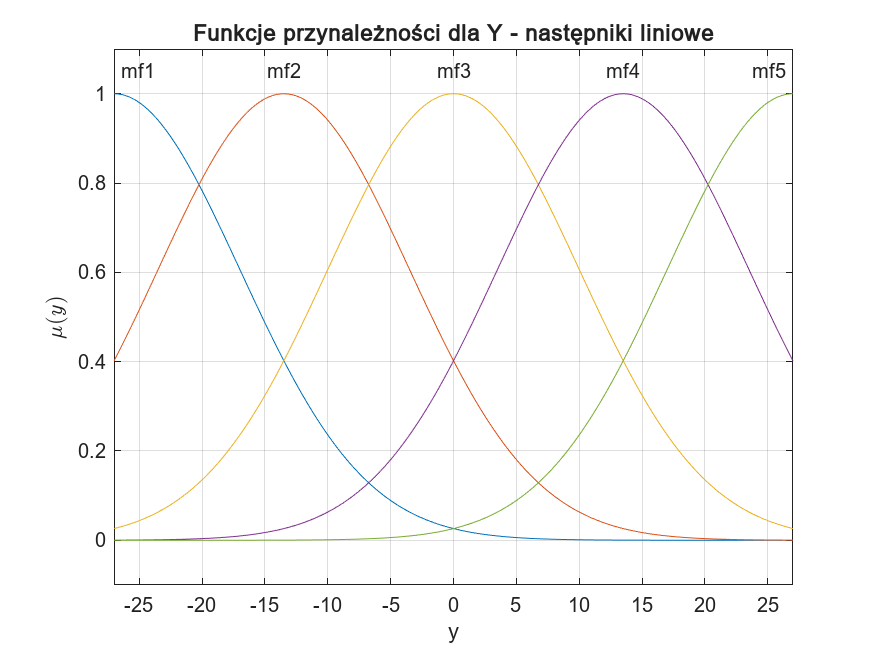
\includegraphics[width=0.85\textwidth]{pictures/WienerfuzzySets_liniowe}
\caption{Zbiory rozmyte - następniki liniowe.}
\end{figure}

\vfill

\begin{figure}[h!]
\centering
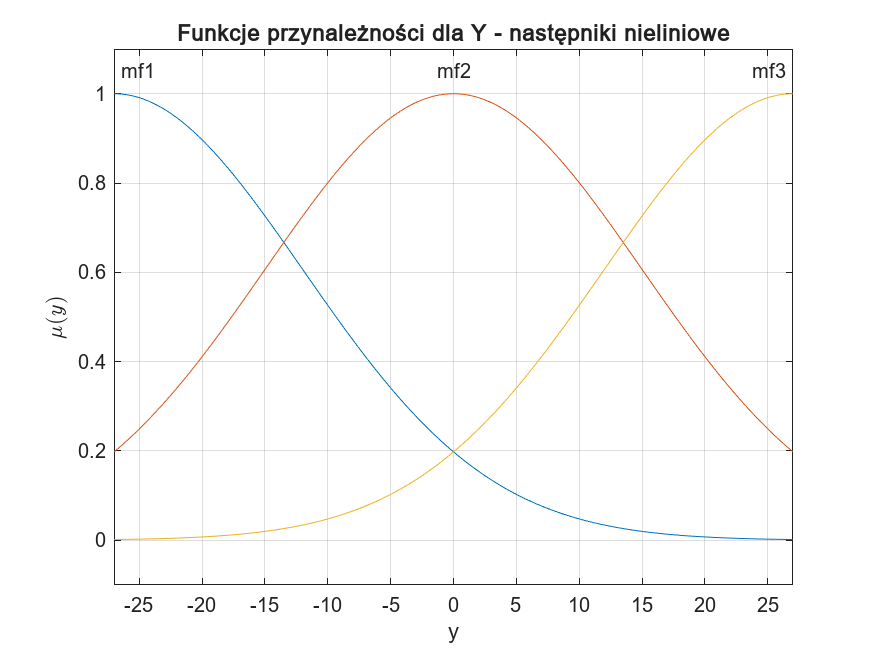
\includegraphics[width=0.85\textwidth]{pictures/WienerfuzzySets_nieliniowe}
\caption{Zbiory rozmyte - następniki nieliniowe.}
\end{figure}

\newpage

\subsection{Porównanie}

Procedura porównawcza wyglądała identycznie jak w przypadku modelu Hammersteina, tj. dla tych samych wygenerowanych sekwencji sygnału sterującego wyznaczono odpowiedzi modelu nieliniowego, liniowego, modelu Wienera z następnikami liniowymi oraz hiperbolicznymi. Przebiegi przedstawiono na rys. \ref{first_wien} - \ref{last_wien}, natomiast dane liczbowe zgromadzono w tab. \ref{comparison_wien}.

\begin{figure}[h!]
\centering
\subfloat[Następniki liniowe]{
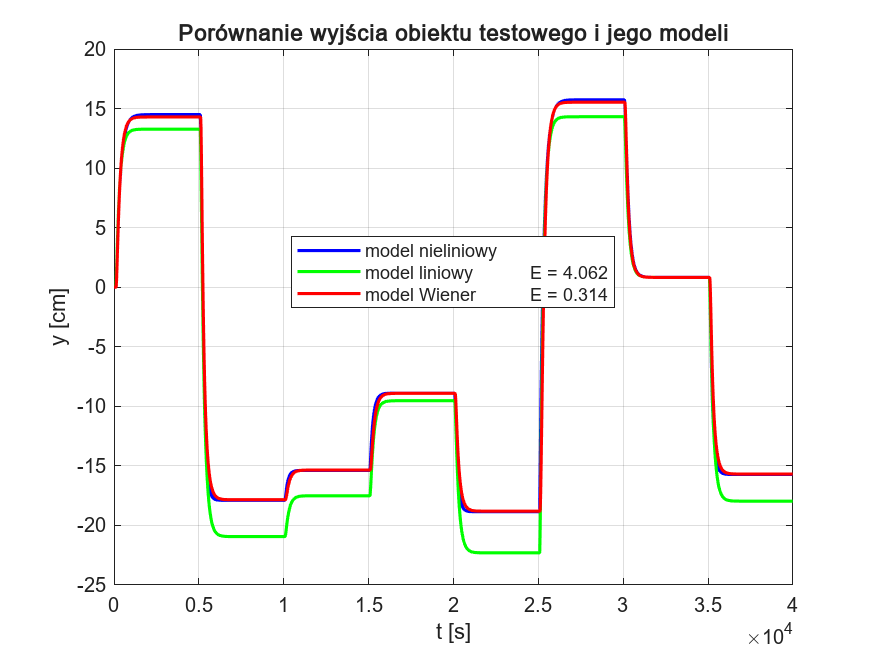
\includegraphics[width=0.7\textwidth]{pictures/WienerLinearModel_1}}
\vspace{0.5cm}
\subfloat[Następniki nieliniowe]{
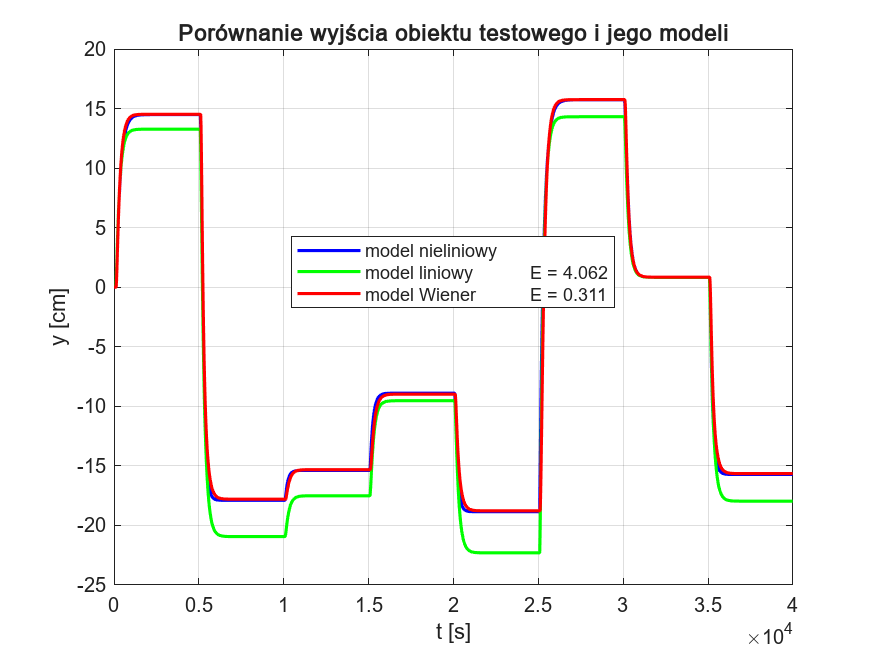
\includegraphics[width=0.7\textwidth]{pictures/WienerNonlinearModel_1}}
\caption{Porównanie modelu Wienera z następnikami liniowymi i nieliniowymi - pierwsza sekwencja.}
\label{first_wien}
\end{figure}

\begin{figure}[p]
\centering
\subfloat[Następniki liniowe]{
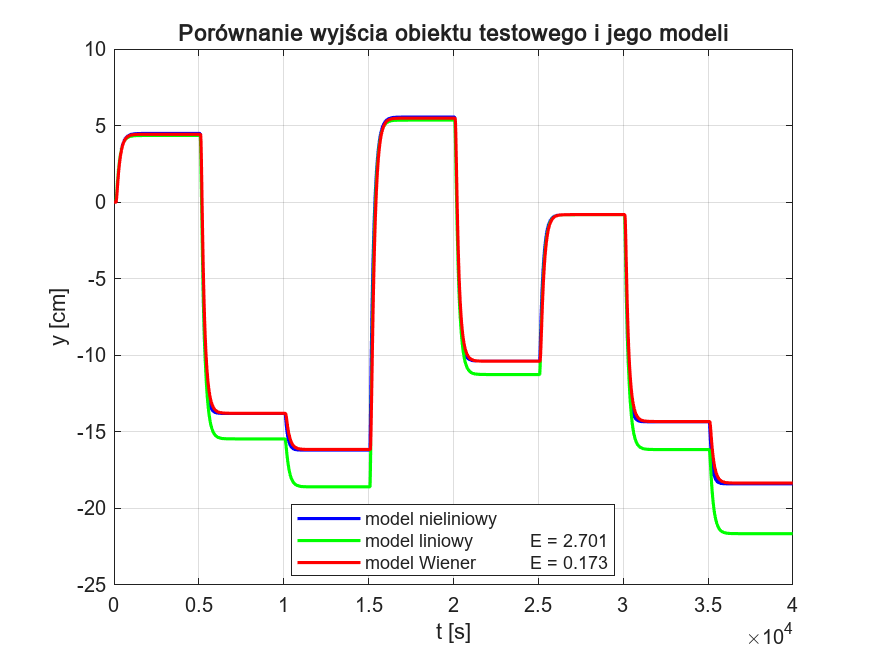
\includegraphics[width=0.75\textwidth]{pictures/WienerLinearModel_2}}
\vspace{0.5cm}
\subfloat[Następniki nieliniowe]{
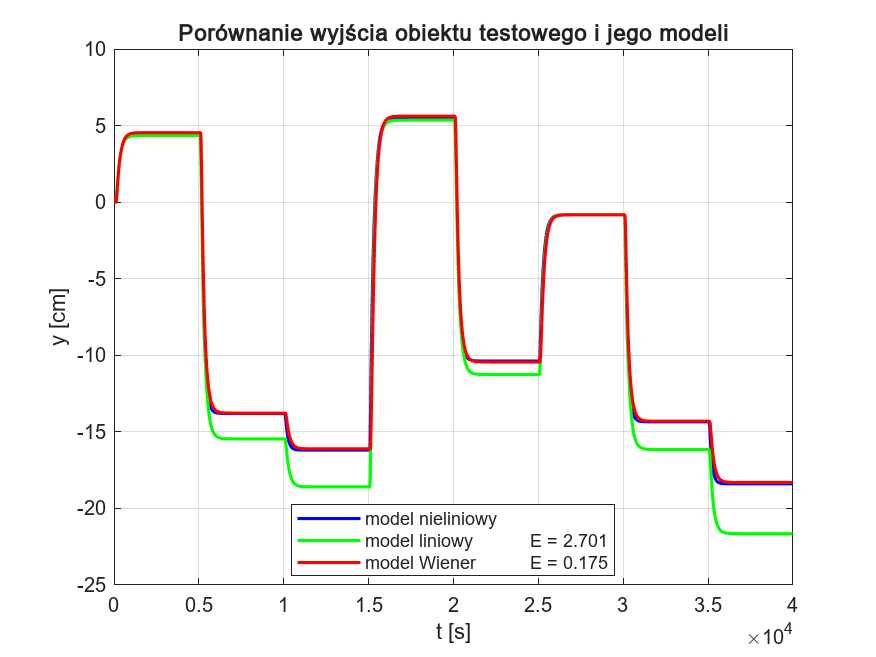
\includegraphics[width=0.75\textwidth]{pictures/WienerNonlinearModel_2}}
\caption{Porównanie modelu Wienera z następnikami liniowymi i nieliniowymi - druga sekwencja.}
\end{figure}

\begin{figure}[p]
\centering
\subfloat[Następniki liniowe]{
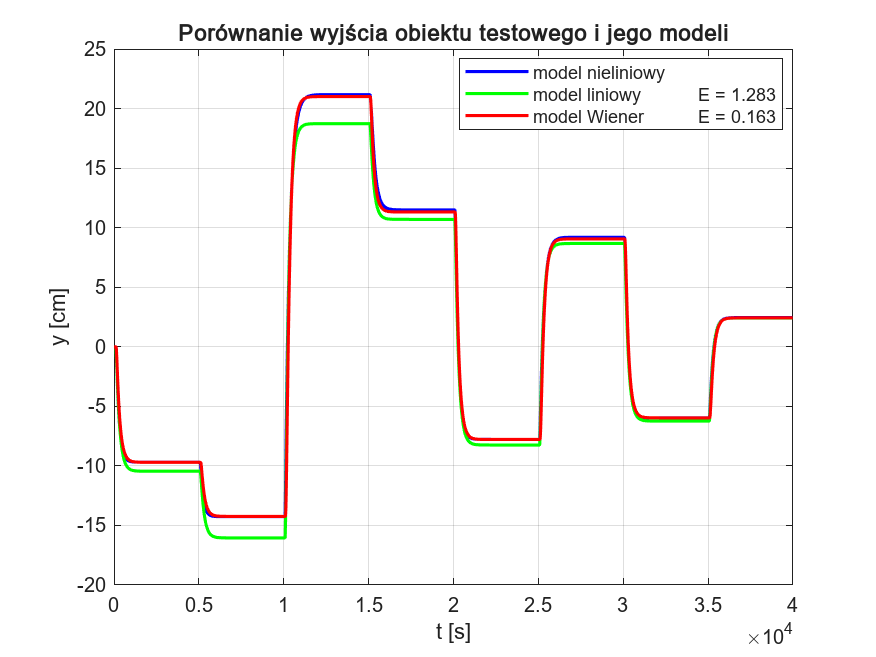
\includegraphics[width=0.75\textwidth]{pictures/WienerLinearModel_3}}
\vspace{0.5cm}
\subfloat[Następniki nieliniowe]{
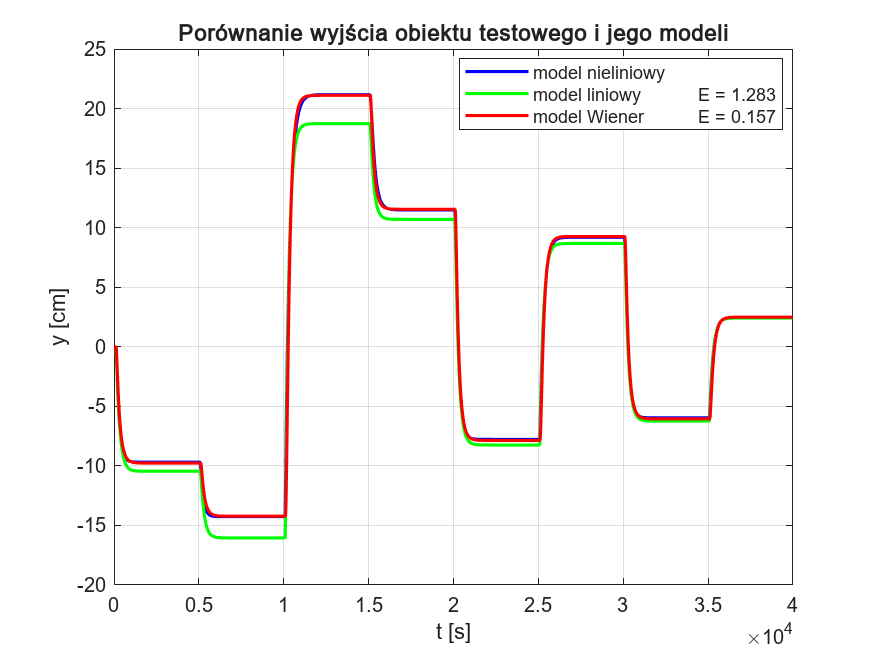
\includegraphics[width=0.75\textwidth]{pictures/WienerNonlinearModel_3}}
\caption{Porównanie modelu Wienera z następnikami liniowymi i nieliniowymi - trzecia sekwencja.}
\end{figure}

\begin{figure}[p]
\centering
\subfloat[Następniki liniowe]{
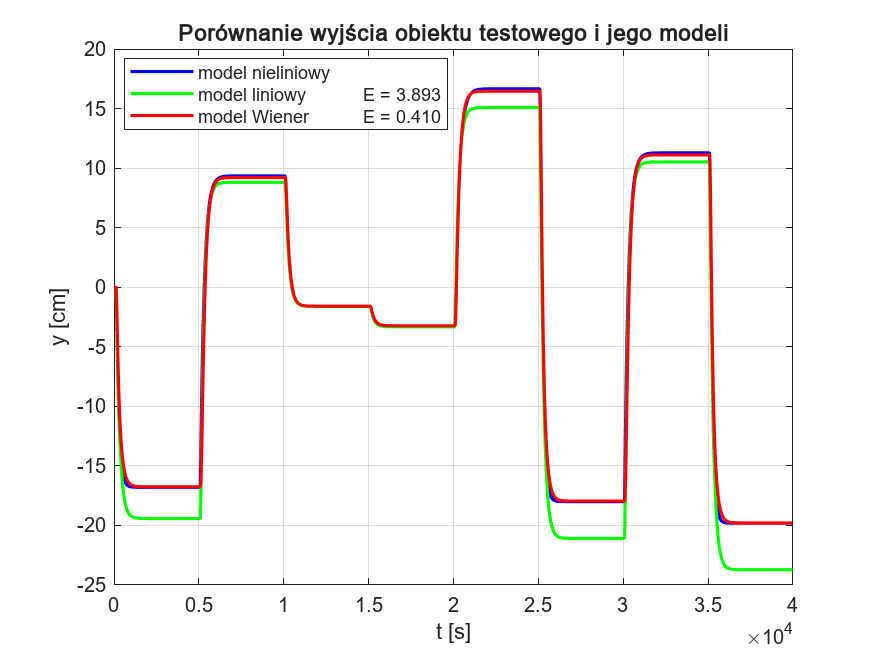
\includegraphics[width=0.75\textwidth]{pictures/WienerLinearModel_4}}
\vspace{0.5cm}
\subfloat[Następniki nieliniowe]{
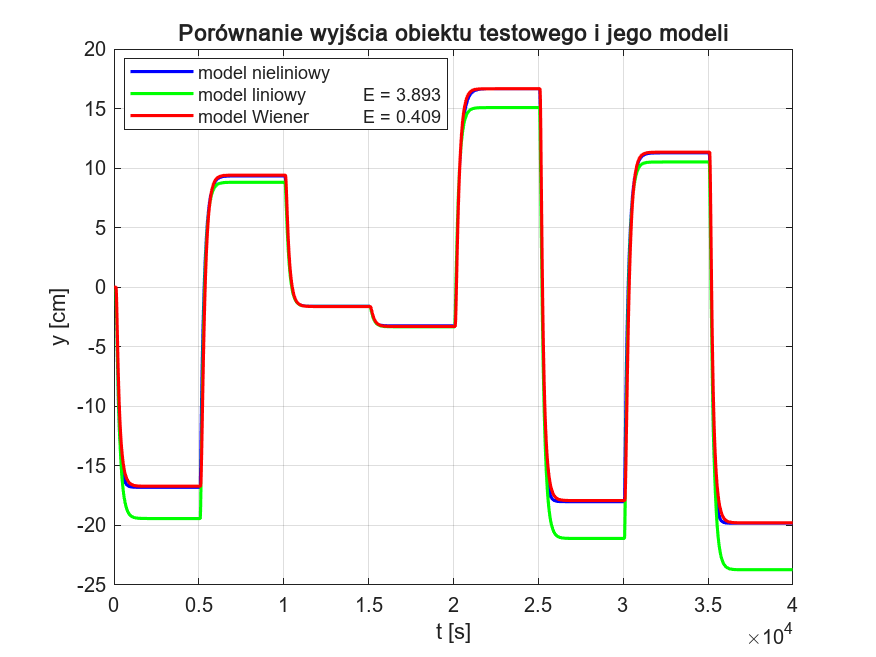
\includegraphics[width=0.75\textwidth]{pictures/WienerNonlinearModel_4}}
\caption{Porównanie modelu Wienera z następnikami liniowymi i nieliniowymi - czwarta sekwencja.}
\end{figure}

\begin{figure}[p]
\centering
\subfloat[Następniki liniowe]{
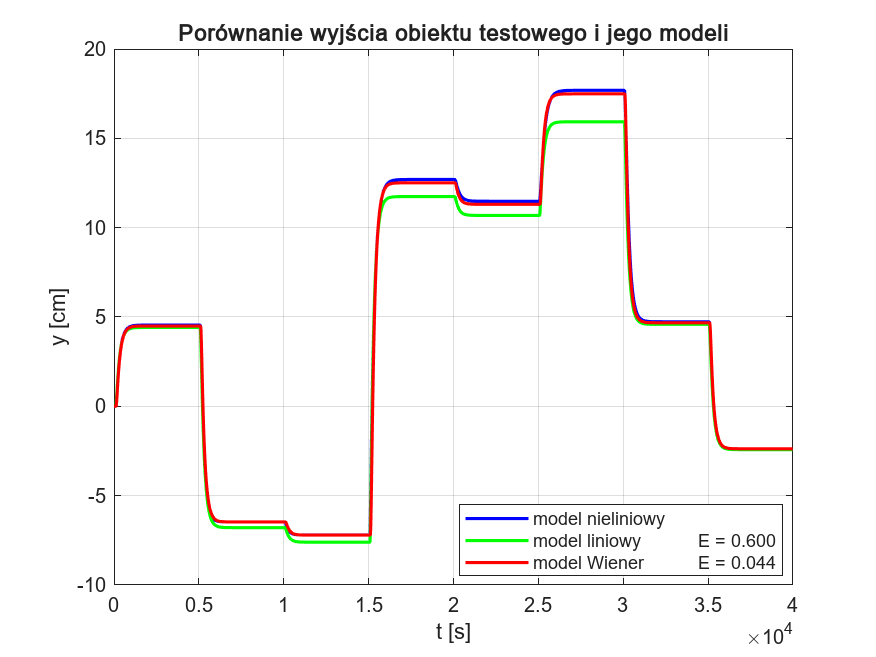
\includegraphics[width=0.75\textwidth]{pictures/WienerLinearModel_5}}
\vspace{0.5cm}
\subfloat[Następniki nieliniowe]{
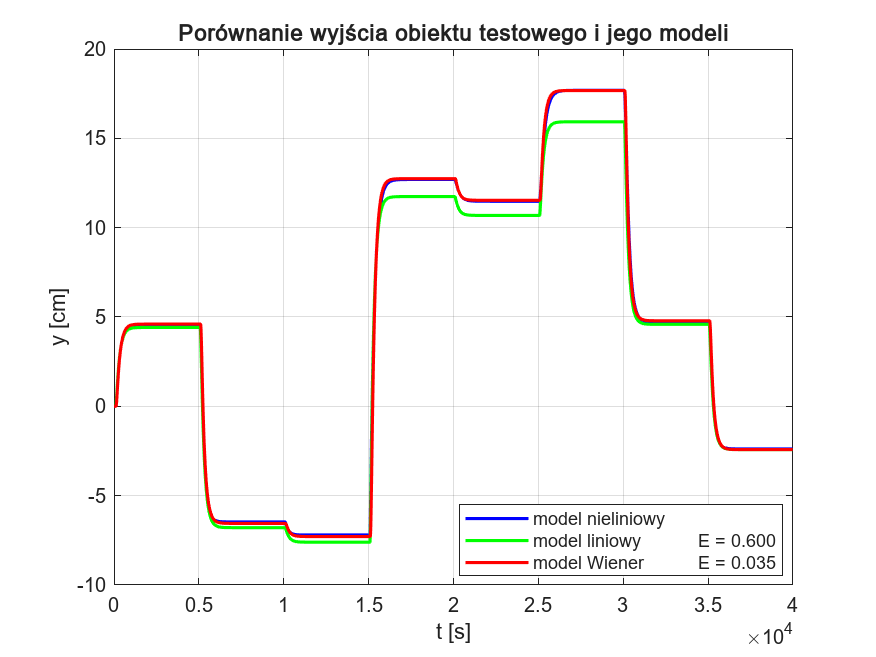
\includegraphics[width=0.75\textwidth]{pictures/WienerNonlinearModel_5}}
\caption{Porównanie modelu Wienera z następnikami liniowymi i nieliniowymi - piąta sekw encja.}
\label{last_wien}
\end{figure}

\newpage

Wyniki zebrane w tab. \ref{comparison_wien} dla modelu Wienera z następnikami liniowymi i nieliniowymi są niemalże identyczne, a ewentualne różnice są pomijalne. Porównując otrzymane rezultaty z tymi otrzymanymi w przypadku modelu Hammersteina okazuje się, że model Wienera jest nieco lepszy, co może wskazywać na większe nieliniowości na wyjściu procesu.
 
\begin{table}[h!]
\centering
\renewcommand{\arraystretch}{1.2}
\begin{tabular}{|>{\centering\arraybackslash}m{2cm}|>{\centering\arraybackslash}m{3cm}|>{\centering\arraybackslash}m{3cm}|>{\centering\arraybackslash}m{3cm}|}
\hline
\multirow{2}{*}{Nr sekwencji} & \multirow{2}{*}{Model liniowy} & \multicolumn{2}{c|}{Model Wienera} \\ \cline{3-4}
 &  & Następniki liniowe & Następniki nieliniowe \\ \hline
1. & $\num{4.062}$ & $\num{0.314}$ & $\num{0.311}$ \\ \hline
2. & $\num{2.701}$ & $\num{0.173}$ & $\num{0.175}$ \\ \hline
3. & $\num{1.283}$ & $\num{0.163}$ & $\num{0.157}$ \\ \hline
4. & $\num{3.893}$ & $\num{0.410}$ & $\num{0.409}$ \\ \hline
5. & $\num{0.600}$ & $\num{0.044}$ & $\num{0.035}$ \\ \hline
\end{tabular}
\caption{Porównanie modeli.}
\label{comparison_wien}
\end{table}

Udało się osiągnąć zamierzony efekt - mniejsza liczba reguł, bez utraty dokładności.